\section{Base de datos}


\subsection{Introducción}
\label{}
Mencionar que tipo de base de datos se necesita encontrar\\
Con el fin de relevar distinta clases de actividades humanas y en particular la marcha, se pretende trabajar con una base de datos basada en marcadores, que contenga un cierto número de sujetos, realizando una variedad de movimientos predefinidos, donde para cada sujeto a estudiar, se tengan múltiples secuencias de videos 2D del movimiento obtenidas a partir de cámaras situadas en un entorno 3D cerrado previamente acondicionado. Dicha base debe contar con el correspondiente ground truth 2D y 3D de los datos de movimiento relevados, en nuestro caso como nuestro sistema está basado en marcadores, dicha información consiste en obtener las coordenadas espaciales a lo largo del tiempo para cada marcador de interés. Así como la información de calibración.blablabla MEJORAR \\

Mencionar porque se tuvo que generar una y que contiene a grandes rasgos.\\
Se propone una estructura de datos para almacenar la información relevante del ground truth y  se cuenta con código de soporte que facilita la generación de nuevas secuencias así como la gestión de la información en la estructura de datos, evaluar resultados y realizar el  posterior análisis de performance.


blablablabl
Un ambiente controlado con cámaras ajustadas convenientemente provee un escenario ideal para obtener información óptica de los marcadores. El sujeto es condicionado a moverse sobre un espacio de captura determinado con una vestimenta particular; la elección adecuada de estos parámetros junto con las condiciones de iluminación y el tipo de fondo facilitan la recolección de información, el posterior análisis y sobre todo la performance del sistema completo.
\\COMBINAR LO ANTERIOR CON ESTO
Necesitamos una base de datos para implementar, testear y comparar los distintos tipos de algoritmos desarrollados. Por lo tanto es de interés primario relevar las bases de datos existentes o en su defecto realizar una.\\
Para ello en primera instancia se buscaron bases de datos en la web. La búsqueda se centro en encontrar secuencias de video de personas caminando donde, dada las características de nuestro proyecto, las mismas deben poseer marcadores claramente distinguibles. Las secuencias deben ser tomadas con varias cámaras ubicadas alrededor del sujeto y para obtener información 3D como mínimo la cantidad de cámaras deben ser dos. Además se debe tener el ground truth con la posición espacial de dichos marcadores para testear y comparar los distintos algoritmos de seguimiento aplicados sobre dichas secuencias


\subsection{Revisión de base de datos}
\label{}
En esta sección se muestra  resultados del relevamiento de bases de datos útiles para el análisis de la marcha.
Inicialmente nuestro objetivo era obtener un sistema funcional para el caso de la marcha humana, aunque luego de la implementación del mismo se generalizaron sus usos, las bases de datos con este tipo de movimiento fueron el eje central de la búsqueda.

Se encontraron principalmente tres páginas web que a manera de compendio agrupan  bases de datos útiles en varias de las ramas de la visión por computadora.\\

\hspace{-0.7cm} \textbf{CVonline \footnote{\textcolor{blue}{\underline{\url{http://homepages.inf.ed.ac.uk/rbf/CVonline}}}. Accedido 30-11-14.} } 

Bastante completa, no solo contiene enlaces a  varias bases de datos sino reune bibliografía e implementaciones útiles.\\


\hspace{-0.7cm} \textbf{Computer Vision Papers \footnote{\textcolor{blue}{\underline{\url{ http://www.cvpapers.com/datasets.html}}}. Accedido 30-11-14.} } 

	 Solo reúne enlaces de bases de datos.\\
		

\hspace{-0.7cm} \textbf{Yet Another Computer Vision Index To Datasets (YACVID)} \footnote{\textcolor{blue}{\underline{\url{http://riemenschneider.hayko.at/vision/dataset/}}}. Accedido 30-11-14. } 	

Una característica importante es que la página contiene direcciones a bases de datos relativamente nuevas y resalta aquellas que son usadas con mayor frecuencia. \\
	

Dentro de estas páginas se encuentra una gran variedad de bases de datos que tratan el caso particular de la marcha, en la tabla \ref{bases_relevadas} se muestran algunas de las bases relevadas y sus características representativas, que permiten hacer una idea del panorama global encontrado a la hora de recopilar información en la web.  

\begin{table}[h!]
	\centering	
	\caption{Comparación de algunas bases de datos disponibles y empleadas por la comunidad.}
	\label{bases_relevadas}
	\begin{minipage}{\textwidth} %por algún motivo el arabic no funciona, no me pone llamados a pie de página numericos	
	\begin{tabular}{||l|ccccc||} 
\hline
\rowcolor[HTML]{CBCEFB} 

\textbf{Base}     & \textbf{Cantidad }  & \textbf{Nro. de }   & \textbf{Entorno} & \textbf{Número de} & \textbf{Calibración}\\
\rowcolor[HTML]{CBCEFB} 
\textbf{de datos} & \textbf{de sujetos} & \textbf{secuencias} &         & \textbf{cámaras }  &  \textbf{disponible} \\


\hline \hline
M.C.L.\footnote{Motion Capture Lab}  & 3 		& 		299	   & Interior&     1    &    No      \\ \hline
C.M.U  \footnote{Carnegie Mellon University Motion Capture Database}	
 & >100     &       2605   & Interior&      1   &    No       \\ \hline
G.T \footnote{Georgia Tech} &       20    & $\sim$100           & Interior y &   3      &  Si       \\ 
	 &		 &					 & exterior        &         &    \\ \hline
U.S. \footnote{University of Southampton Database} &       >100    &     $\sim$       & Interior &   12      &  $\sim$      \\ \hline
Human ID  &     122    & 1870           & Exterior &   2      &$\sim$       \\ \hline
HumanEva &     4+2    & 56           & Interior &   4/7      &  Si       \\ \hline
INRIA \footnote{INRIA Perception, Multicam Dataset. } &       >11    & >40           & Interior &   $\geq$1      &  Si       \\ \hline
CMU Mobo \footnote{CMU Motion of Body.} &     25    & 100           & Caminadora &   6      &  $\sim$       \\ \hline
CASIA &     385    & $\sim$           & Interior y  &   >4      &  $\sim$       \\ 
&         &            & exterior  &         &      \\ \hline
MHAD \footnote{Berkeley Multimodal Human Action Database.} & 12         & 660            & interior  & 12        & Si      \\ 
\hline \hline


\rowcolor[HTML]{CBCEFB}
\textbf{Base}     & \textbf{Movimientos}  & \textbf{Apariencia}    & \textbf{Ground Truth} & \textbf{Tipo}  & \\
\rowcolor[HTML]{CBCEFB}
\textbf{de datos} & \textbf{disponibles} &               &           & \textbf{de acceso} & \\
\hline \hline
{M.C.L. }   & Varios    &  Traje MoCap & 3D-Vicon \footnote{ Esta notación indica que la captura considerada ground truth, se hizo con un sistema  de captura de movimiento (MoCap) de Vicon-Peak, \textcolor{blue}{\underline{\url{http://www.vicon.com/}}} } & Libre & \\ \hline
{C.M.U }    & Varios    &  Traje MoCap & 3D-Vicon \footnote{Secuencias bvh de CMU, \textcolor{blue}{\underline{\url{http://sites.google.com/a/cgspeed.com/cgspeed/motion-capture}}}.} & & \\ \hline
{G.T} &     Marcha fuera&     Traje MoCap y       & 3D  en formato & Libre & \\ 
 &	   de régimen  &  Natural   &   Maya & & \\ \hline
U.S. &       Marcha    &  Natural    &  $\sim$ & Libre&       \\	\hline
Human ID &     Marcha    & Natural  & $\sim$ & Bajo  &       \\ 
						 &        &   &  & solicitud &       \\ \hline
HumanEva &     Varios    & Natural  & 3D - Vicon & Bajo  &       \\ 
						 &        &   &  & solicitud &       \\ \hline
INRIA &       Varios    & Traje MoCap y            & 2D - MoCap &  Libre &       \\
&           & Natural            &   etiquetado manual  & &         \\ \hline
CMU Mobo &     5 tipos de marcha    & $\sim$           & Etiquetado Manual \footnote{Disponible en  \textcolor{blue}{\underline{\url{http://www.cs.cmu.edu/~zhangjy/\# Data}}}.}& Bajo  &       \\ 
 							 &        &   &  & solicitud &       \\ \hline
CASIA &  Varias velocidades       &   Natural         & No  &    Bajo     &      \\ 
& de marcha        &            &   & solicitud        &      \\ \hline
MHAD & Varios        & Traje MoCap            & 3D - Impulse \footnote{ Esta notación indica que la captura considerada ground truth, se hizo con un sistema  de captura de movimiento (MoCap) Impulse (PhaseSpace Inc., San Leandro, CA), \textcolor{blue}{\underline{\url{http://www.phasespace.com/}}} }    & Libre  &       \\
\hline
	\end{tabular}
	\end{minipage}	
\end{table}

A continuación algunos comentarios que vale la pena resaltar sobre  las bases anteriores.

\paragraph{Motion Capture Lab.\footnote{\textcolor{blue}{\underline{\url{http://accad.osu.edu/research/mocap/mocap_home.htm}}}. Accedido 30-11-14}} 
		Como describe el nombre, este laboratorio se centra en obtener capturas de movimiento tridimensionales a través del sistema Vicon. Cuentan con un sistema Vicon 8i de 14 cámaras, dos videocámaras digitales Sony DSR-PD150 que llegan a 30 fps\footnote{\textcolor{blue}{\underline{\url{http://www.bhphotovideo.com/c/product/197878-REG/Sony_DSRPD150_DSR_PD150_Professional_1_3_DVCAM.html}}} ,Accedido 29-11-14 }, junto a un sistema de sincronización que permite integrar todas estas cámaras en el laboratorio. El video se utiliza únicamente como ayuda en los datos de captura para corregir y ver los marcadores,  por lo que \underline{no cuenta con secuencias de video adecuadas}. Cabe destacar que maneja múltiples formatos MoCap, inclusive el bvh.

\paragraph{Carnegie Mellon University Motion Capture Database.\footnote{\textcolor{blue}{\underline{\url{http://mocap.cs.cmu.edu/}}}. Accedido 30-11-14}}
 Este laboratorio también se centra en obtener capturas de movimiento a través de un sistema Vicon, y no está implementado para evaluaciones ópticas de las capturas. Solo maneja videos monoculares de baja resolución, por lo que no cuenta con secuencias de video adecuadas para nuestro proyecto. Sin embargo maneja múltiples formatos MoCap y  posee herramientas para conversión a otros formatos, incluido el bvh. Posee descripción detallada de la ubicación de los marcadores, así como de la configuración del laboratorio. El sujeto a relevar se encuentra vestido con ropas finas y ajustadas, sobre la cual se colocan los marcadores, por lo tanto se puede despreciar las fluctuaciones de posición de marcadores debidas a la ropa, que si exhiben otros ambientes menos controlados  Esta base de datos es bastante utilizada en el ámbito de la  animación por computadora y es por lejos la que dispone de mayor cantidad de capturas de movimiento de acceso público de las bases relevadas en esta sección.

\paragraph{Georgia Tech.\footnote{\textcolor{blue}{\underline{\url{http://www.cc.gatech.edu/cpl/projects/hid/index.html}}}. Accedido 30-11-14}}
Se encuentra desarrollando maneras de identificar a los seres humanos a distancia a través del reconocimiento de la marcha. También llevan a cabo trabajos relacionados en la localización y seguimiento de rostros, la detección de oclusiones y actividades específicas de sustracción de fondo.
Lamentablemente las cámaras están todas sobre un costado del caminante, la resolución es baja y no todos los videos poseen marcadores. No se cuidan las condiciones de laboratorio para trabajar de manera óptica según nuestras necesidades.


\paragraph{University of Southampton Database.\footnote{ \textcolor{blue}{\underline{\url{http://www.gait.ecs.soton.ac.uk/database}}}. Accedido 30-11-14}}
Interesados en el reconocimiento de personas a través del seguimiento de la marcha, relevantes sobre todo por ser pioneros en el estudio biomecánico de la marcha. Poseen dos bases de datos, HiD gait database  (100 sujetos) y Biometric tunnel. El servidor donde se alojaba la base de datos está fuera de línea desde el 2004, el encargado de la página es Mark Nixon (\textcolor{blue}{\underline{\url{msn@ecs.soton.ac.uk}}}). Aparentemente se continúa actualmente el proyecto en \textcolor{blue}{\underline{\url{http://www.cspc.ecs.soton.ac.uk/gait}}}\footnote{Accedido 30-11-14}. Si bien estas bases de datos no están basadas en marcadores, cabe resaltar que el fondo del espacio de captura del túnel biométrico contiene patrones asimétricos con colores saturados que facilitan no solo la extracción de fondo sino también la automatización del proceso de calibración.

\paragraph{Human ID Gait Challenge Dataset.\footnote{\textcolor{blue}{\underline{\url{http://marathon.csee.usf.edu/GaitBaseline/ }}}. Accedido 30-11-14} }
Contiene 1.2 Tera bytes de información. Utilizada para el reconocimiento de la marcha,  no posee marcadores. Al igual que en la base de Southampton contiene en la secuencia imágenes de dameros convenientemente dispuestos, útiles para calibrar las cámaras. Las sucesivas secuencias tomadas para un mismo sujeto modifican distintos tipos de factores, como la calidad del terreno a recorrer, si el sujeto lleva o no un maletín y el  tipo de calzado utilizado. Tienen disponible junto a todas las secuencias de la base de datos las siluetas de los sujetos, obtenidas con un algoritmo base también propuesto y disponible. Lamentablemente el enlace que indica el protocolo seguido para obtener secuencias, junto con la especificación del equipamiento, está fuera de línea.

\paragraph{HumanEva.\footnote{\textcolor{blue}{\underline{\url{http://vision.cs.brown.edu/humaneva/index.html }}}. Accedido 30-11-14} \cite{humaneva} }
Con solo 13 Gigabit de información, el trabajo de este laboratorio es muy completo, incluye métricas de evaluación y un análisis importante de las necesidades actuales a la hora de generar una base de datos para relevar actividades humanas. El único inconveniente para cumplir los requisitos de nuestro proyecto es que no está pensado para el seguimiento óptico de marcadores, por lo que los marcadores sobre los sujetos de estudio utilizados para recabar datos Mocap son escasos y demasiado pequeños, las condiciones de luminosidad y color de fondo no son las adecuadas para nuestro propósito, incluso utilizan máscaras sobre las imágenes ópticas para cubrir los marcadores, estos últimos son utilizados solo para recopilar el ground truth a través de un sistema Vicon.  Dado que su motivación es obtener una imagen ``natural'' del sujeto que contenga la complejidad generada por el movimiento de la ropa, el ground truth que presentan  no es tan preciso como los obtenidos por métodos más tradicionales.  Contiene código para efectuar sustracción de fondo y la implementación de un algoritmo base, con un filtrado de partículas utilizado para el seguimiento de la pose del sujeto. Para acceder a los datos se debe gestionar un permiso en la página de HumanEva. 

\paragraph{INRIA Perception, Multicam Dataset.\footnote{INRIA Perception, Multicam Dataset, \textcolor{blue}{\underline{\url{http://4drepository.inrialpes.fr/pages/home}}}. Accedido 30-11-14}} Efectúan las capturas con múltiples cámaras y también ofrecen la secuencia de malla de los sujetos reconstruidos a partir de las imágenes. Ofrecen un software que permite navegar en 4D, es decir, el espacio y el tiempo, sobre los modelos disponibles en su base de datos. Por lo que estos modelos se pueden ver desde cualquier ángulo de visión e inspeccionar congelándolos en cualquier instante de tiempo. Lamentablemente su captura no está basada en marcadores. 

\paragraph{CMU MoBo Dataset.\footnote{CMU Motion of Body,  \textcolor{blue}{\underline{\url{http://www.ri.cmu.edu/publication_view.html?pub_id=3904}}}. Accedido 30-11-14}}
Estudia la marcha humana, enfocada en la identificación Biométrica de humanos a partir de sus características individuales. Los sujetos bajo estudio efectúan 4 tipos de caminata sobre una caminadora: marcha lenta, marcha rápida, marcha sobre plano inclinado y marcha sosteniendo un balón. Se utilizan 6 cámaras de alta resolución ubicadas alrededor de la caminadora que adquieren imagenes a 30 frames/s. Para acceder a la base de datos debe pedirse acceso comunicandose con \textcolor{blue}{\underline{\url{rgross@cs.cmu.edu }}}

\paragraph{CASIA Gait Database.\footnote{ \textcolor{blue}{\underline{\url{http://www.cbsr.ia.ac.cn/english/Gait\%20Databases.asp
 }}}. Accedido 30-11-14}} 
Contiene 4 bases de datos sobre la marcha, la primera se efectúa en exteriores y posee una sola cámara; la segunda es en interiores  y posee 11 cámaras sobre un lado del sujeto; la tercera utiliza cámaras infrarrojas y cada sujeto efectúa tres tipo de marcha, lenta, rápida y con mochila; por último la cuarta combina la información de cámaras de captura con una plataforma que registra la presión de la planta del pie a medida que el sujeto desarrolla el movimiento. Además de los archivos de vídeo, ofrecen las siluetas humanas a partir de sus secuencias de vídeo. Las capturas visuales no están basadas en marcadores.

\paragraph{Berkeley Multimodal Human Action Database (MHAD).\footnote{\textcolor{blue}{\underline{\url{http://tele-immersion.citris-uc.org/berkeley_mhad\#dl  }}}. Accedido 30-11-14}}
El objetivo de esta base de datos es reconocer el movimiento del cuerpo al realizar este distintas actividades. Tiene la información necesaria para efectuar sustracción de fondo, devuelven información desde múltiples fuentes:
\begin{itemize}
\item sistema con 12 cámaras ópticas agrupadas en 4 conjuntos de cámaras estéreo
\item dos sensores Kinect
\item 6 acelerómetros sobre el sujeto
\item 4 micrófonos a cada lado del espacio de captura
\end{itemize} Todas estas fuentes se encuentran sincronizadas. Esta base de datos es bastante completa en cuanto a los tipos de captura que realiza, pero los marcadores utilizados son leds y únicamente se utilizan para recabar información para el ground truth, con lo cual no se cuida de obtener una buena información óptica de los mismos. 



\subsubsection{Contactos realizados y resultados}

En el ámbito local hemos estado en contacto con magister Patricia Polero y xxxxx del hospital de clínicas, quienes actualmente poseen un sistema de captura de movimiento basado eb xxx el cual han adquirido recientemente. Explicar porque no lo usamos!!!!
Hablar también de la gente del clínicas y de Patricia Polero
JUSTIFICAR LA ELECCION DE LOS PEDIDOS
Los pedidos fueron realizados el 17 de diciembre de 2013 aproximadamente.


\begin{table}[h!]
	\centering		
	\begin{tabular}{@{}lr@{}} 
	\toprule		
	\multicolumn{1}{l}{\textbf{Base de datos}} & \textbf{Resultados }\\	
	\midrule
	HumanEva		&	concedida 27 julio 2014\\
	CASIA			&	concedida 3 de mayo 2014\\
	CMU Mobo		&	sin respuesta \\
	\midrule
	\multicolumn{1}{l}{\textbf{Escasas secuencias de video}} & \textbf{Resultados }\\
	\begin{tabular}[l]{@{}l@{}}Darío Santos,\\ Depto. Fisiatría Y
	Rehabilitación.\\ Hospital de Clínicas.\end{tabular}	&	concedida 29 julio 2014\\	
	\bottomrule
	\end{tabular}
	\caption{Solicitudes de acceso gestionadas.}
	\label{solicitudes}	
\end{table}



\subsubsection{Conclusiones}

Si bien se encontraron numerosas bases de datos para la marcha, todas ellas terminan siendo descartadas por no ajustarse completamente a las hipótesis bajo las cuales se trabaja en este proyecto. Deficiencias tales como la inadecuada cantidad o posición de las cámaras, condiciones del laboratorio que dificultan y en algunos casos imposibilitan una correcta segmentación a partir de la información óptica. Y por último la ausencia o tamaño inadecuado de los marcadores. Son los factores más importantes.
Salvando diferencias, el problema principal está en que no se tienen imágenes ópticas para trabajar con marcadores, en general se tiende a trabajar sobre el cuerpo completo, y se contrasta el procesamiento con datos Mocap relevados con sistemas infrarrojos. Por otro lado esto último genera una rica fuente de material de trayectorias de puntos en distinto tipo de movimientos, sobre todo en formatos Mocap.
Estas consideraciones impulsaron la idea de recorrer el camino inverso, crear una base de datos sintética a partir del material Mocap disponible, para luego generar los videos en los cuales trabajar.  







Si bien la búsqueda se centró en blablabla no logró encontrar una base de datos que cumpliera las especificaciones de nuestro proyecto. Debido a blablabla SEGUIMIENTO OPTICO DE MARCADORES.
 De todas maneras se genera un relevamiento de bases de datos para el movimiento humano, se profundiza en las características usuales que presentan dichas bases de datos y se logra reunir un conjunto de conceptos y herramientas necesarios para introducirnos en el tema. 

% % % % % % % % % % % % % % % % % % % % % % % % % % % % % % % % % % % % % % % % % % % % % % % % % % % % % % % % % %
% % % % % % % % % % % % % % % % % % % % % % % % % % % % % % % % % % % % % % % % % % % % % % % % % % % % % % % % % % %5


\subsection{Características de Laboratorio para un sistema de captura óptica basado en marcadores}
\subsubsection{Variables}
 
A continuación se enumeran un cierto número de variables que es necesario tener en cuenta a la hora de diseñar un Laboratorio, adecuado para un sistema de captura basado en marcadores. También se discute brevemente el posible impacto de estás variables en el tratamiento posterior de las secuencias.

\paragraph{Cámaras} 
Para la elección del tipo de cámaras es importante tener en cuenta los requerimientos de las secuencias a relevar. A continuación vamos a tratar dos variables básicas y generales que deben contemplarse, por un lado la cantidad de fotogramas, y por otro la resolución de la cámara.

La cantidad de fotogramas por segundo de las secuencias de video condiciona la resolución temporal de los datos procesados a partir de dichas secuencias, así como también limita la velocidad de movimiento a realizar por el sujeto si se busca una captura aceptable.
Basados en el relevamiento de las distintas bases de datos se puede afirmar que 30fps es un valor normal para trabajar el caso de la marcha, pudiendo obtener en este caso información de la posición de los marcadores solo cada 1/30 segundos.\\ 
Hay que tener presente que si se efectúan movimientos de velocidades superiores a la marcha, manteniendo la cantidad de fotogramas anterior, aumenta la dificultad a la hora de vincular temporalmente los datos obtenidos, pudiendo bajar la performance del seguimiento de los marcadores. 

Respecto a los tiempos de obturación, estos deben ser bastante cortos  para no producir efectos de desplazamiento nocivos a la hora de reconocer los marcadores.
Una regla habitualmente utilizada que sirve de orientación es que el tiempo mínimo de disparo que asegura que no salga movida una imagen, es la inversa de la distancia focal utilizada. También se encuentran referencias que indican los tiempos de obturación recomendados según la actividad a relevar. \footnote{\textcolor{blue}{\underline{\url{http://es.wikipedia.org/wiki/Velocidad_de_obturación}}}}.
\begin{itemize}
\item $1 / 4000~ s$:  se utiliza para tomar fotografías nítidas de sujetos en rápido movimiento, como los atletas o vehículos, en condiciones de buena iluminación.
\item $1 / 2000 ~s$ y $1/ 1000~s$: útil  para fotografías nítidas de sujetos en movimiento moderadamente rápido, bajo condiciones normales de iluminación.
\item $1 / 500~s$ y $1/ 250~s$ :  para tomar fotografías nítidas de personas en movimiento en situaciones cotidianas.
\end{itemize}
 
 
 La resolución del sensor también juega un rol fundamental a la hora de cumplir requerimientos de resolución espacial en los datos de salida.
 En la figura \ref{estimacion_resolucion} se hace un bosquejo que permite estimar la resolución espacial a medida que el sujeto se aleja de la cámara.
 
\begin{figure}[H]
  \centering
  {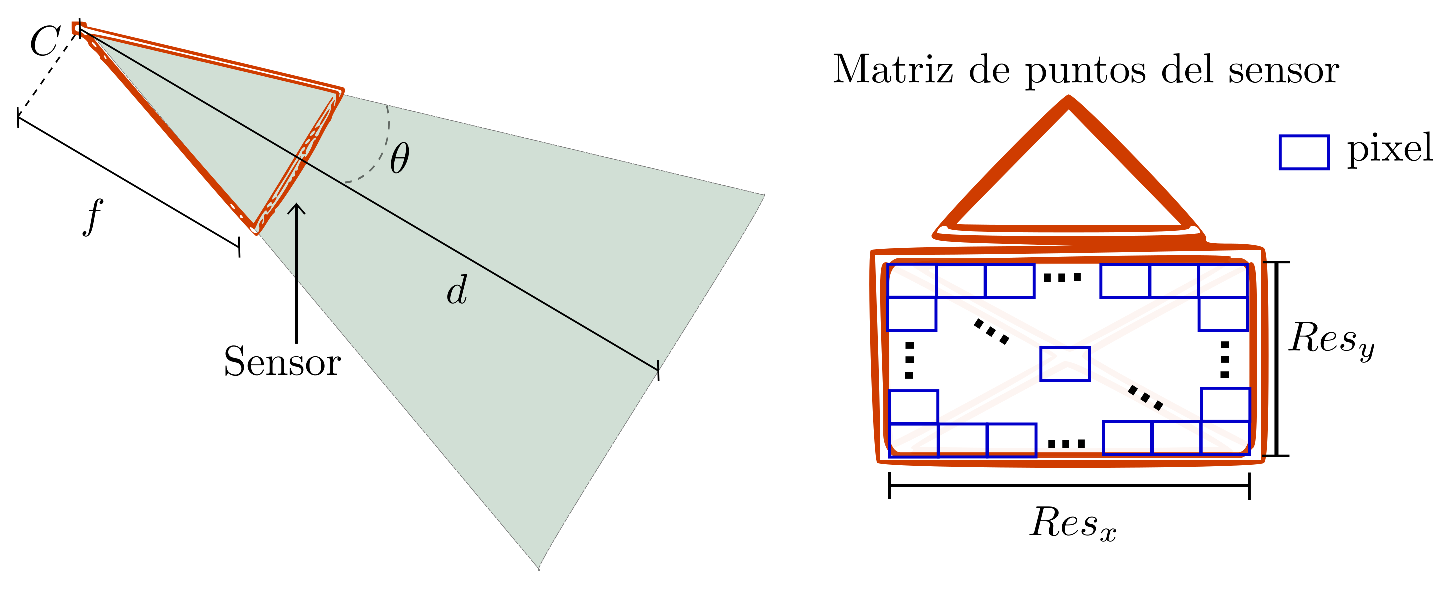
\includegraphics[scale=0.5]{img/Base_Datos/camara_resolucion.eps}\label{peladoOriginalintro}}      
  \caption{Estimación del la resolución espacial.}
  \label{estimacion_resolucion}
\end{figure} 

Llamemos $x_s$ e $y_s$ a magnitudes sobre el sensor de la cámara, horizontal y vertical respectivamente, y sea $X$ e $Y$ las magnitudes a una distancia $d$ del centro $C$ de la cámara que producen respectivamente las proyecciones de magnitud $x$ e $y$ sobre el sensor.
Se cumple la siguiente relación,
\begin{alignat*}{1}
X = \dfrac{d}{f}x_s&~, \quad \quad Y = \dfrac{d}{f}y_s
\end{alignat*}

Si el sensor\footnote{También referido como retina de la cámara.} tiene un largo $S_x$, píxeles cuadrados y resolución de $R_x\times R_y$ píxeles, resulta que la arista de un pixel es $l_p = S_x/R_x $ y el ancho del sensor es $S_y = S_x R_y/ R_x$. 

A modo de ejemplo consideremos una cámara con las siguientes características $S_x = 0.032~m$, píxeles cuadrados, resolución de $1600\times600$ píxeles y una distancia focal de $32~mm$. Por lo tanto un error de un pixel es equivalente a $x = 0,032/1600~m = 0.02~mm$ sobre el sensor. Errores de 1, 2 y 3 píxeles se mapean a una distancia $d$ del centro de la cámara como se muestra en la tabla \ref{table_resolucion} 

\begin{table}[h]
\centering
\begin{tabular}{|c|l|l|l|l|l|}
\hline
\multirow{2}{*}{\begin{tabular}[c]{@{}c@{}}\textbf{número} \\\textbf{ de píxeles}\end{tabular}} & \multicolumn{5}{c|}{\textbf{d (metros)}} \\ \cline{2-6} 
                                                                              &\textbf{ 0,5}  &\textbf{ 1,0}  & \textbf{3,0}  & \textbf{5,0} & \textbf{10,0}\\ \hline
\textbf{1}                                                                             &  0,03    &  0,06    &   0,19   &  0,31   & 0,63      \\ \hline
\textbf{2}                                                                             &  0,06    &  0,12    &  0,38    &  0,62   &  1,26    \\ \hline
\textbf{3}                                                                            &   0,09   &  0,18    &  0,57    & 0,93    &  1.89    \\ \hline
\end{tabular}
\caption{Resolución espacial en centímetros como función de la distancia al centro de la cámara}
\label{table_resolucion}
\end{table}


\paragraph{Marcadores}
A la hora de seleccionar el equipamiento se debe prestar especial atención y coordinar el tipo de marcador, la vestimenta del sujeto, el fondo del espacio de captura y el tipo de iluminación. Pues las características de estos elementos en conjunto pueden cambiar sensiblemente la performance del sistema de captura, sobre todo en sus primeras etapas tales como la detección de marcadores y calibración.
Si se quiere facilitar la tarea de detección automática de marcadores, estos deben ser fácilmente distinguibles del resto del entorno, y visibles la mayor cantidad de tiempo para las cámaras. Para ello se debe tener marcadores que generen un alto contraste con el resto de los elementos dentro de la captura de video. 
Su tamaño y forma también son importantes, por lo general se trabaja con marcadores esféricos, y un tamaño que dado cierto espacio de trabajo no condicione fuertemente la resolución necesaria de las cámaras. Una medida que se puede considerar aceptable con cámaras convencionales y movimientos a menos de 12 metros, son marcadores de $3~cm$ de diámetro.  
Si el fondo del espacio de captura es negro, opaco, al igual que la vestimenta del sujeto a capturar, los marcadores pueden ser blancos, no pulidos de manera que su reflejo sea difuso, para no generar variación de tono sobre los mismos. 
La disposición de los mismos sobre el sujeto responde a los intereses de lo que se quiera observar, pero se debe tener presente que al ser una captura óptica, para que un marcador sea útil, debe estar visibles buena parte del tiempo en la secuencia.

\paragraph{Iluminación}
La iluminación debería ser preferiblemente uniforme, para no generar sombras que modifiquen los tonos del espacio de captura. La luz natural es una buena alternativa, en espacios cerrados lo que habitualmente se utilizan son pantallas delante de los focos lumínicos, en cuanto a la posición depende de la forma del espacio de captura, pero por lo general rodean al mismo, cuidando que los focos no sean capturados  directamente por las cámaras.

\paragraph{Vestimenta}
Es preferible que la vestimenta del sujeto a relevar, consista en ropas finas y ajustadas para despreciar fluctuaciones de la posición de marcadores debido al movimiento de la ropa. Como se menciona anteriormente al igual que el fondo, la elección del color y material debe contrastar con los marcadores.

\paragraph{Espacio de captura}
Las 
-dimensiones del espacio de captura(relacionarlo con la posición de las cámaras y el tipo de movimiento)\\
-fondo del espacio de captura\\
-posición de cámaras (describir como depende del movimiento--marcha-rectilínea, movimiento libre--área circular)\\
-facilidades para calibración\\
Posibilidad: Fondo del espacio de captura con patrones asimeétricos con colores saturados que facilitan la extracción del fondo y la calibración automática.



RECORDATORIO: Aumentar el número de cámaras permite una mayor cobertura de volumen, lo que significa una mayor visibilidad del conjunto de marcadores. A su vez una mejor visibilidad del conjunto de marcadores está correlacionado con disminuir la posibilidad de que los datos importantes se pierdan.


\paragraph{Sincronización \cite{canon}}

Esto resulta esencial en las emisiones con conexiones en directo con varias cámaras, para garantizar que las imágenes de vídeo se mantienen estables incluso cuando se cambia de una cámara a otra.
Se debe contar con un fuente central que envíe una señal de sincronización a todas las videocámaras que participan en una grabación, de esta manera se indica a cada una de ellas cuando deberán comenzar a grabar. La misma orden es enviada para cada fotograma y todas y cada una de las líneas escaneadas dentro del fotograma. El sincronizador ‘bloquea’ las videocámaras en la misma secuencia de escaneado.
Si no se contara con una entrada de sincronización sería prácticamente imposible realizar una grabación con varias cámaras simultáneamente.

\paragraph{Formatos Mocap}
-Formatos Mocap (terminología, ventajas, desventajas, formatos usuales)
\\



\subsubsection{Conclusiones}
especificar los parámetros deseables en una base de datos que trabaje con información óptica basada en marcadores

Notar que trabajando a 10 metros con resolución $1600\times600$ se obtienen incertidumbres de pixel de casi $1 ~cm $

\subsection{Base de datos sintética}
\subsubsection{Motivación}
ACLARAR QUE NO SE CONSIGUIÓ UNA BASE DE DATOS ADECUADA PERO ......RECICLAR LO QUE VIENE

Por otro lado encontramos en el sistema Vicon otra posibilidad. Resulta que la web  ofrece fácilmente un gran número de bases de datos con la captura de movimiento (mocap) de personas realizando diferentes tipo de actividades. Dichas capturas se efectúan por lo general a través de un sistema Vicon, con lo cual se tiene información muy precisa sobre la ubicación 3D de los marcadores ubicados sobre el modelo. El problema radica en que no ofrecen también videos convencionales del modelo efectuando dichas actividades, o sea fácilmente podemos encontrar un ground truth pero no así la secuencia de video que la produce.\\
Esto último tuvo una solución. Las bases de datos con capturas de movimiento son ampliamente utilizadas en animaciones 3D , pues se carga la información de la captura al modelo 3D de interés y este efectúa la acción esperada. Por lo que se vió el potencial que estás capturas de movimiento tienen en el desarrollo de una base de datos sintética.\\
Continuando en esa dirección se trabajo con el programa de animación Blender, generando un modelo 3D con marcadores (el mismo se muestra en la figura \ref{macaco} ) al cual se pretende incorporar la información brindada por las bases de datos de captura de movimiento de interés.  

La principal base de datos utilizada para este fin es CMU (Graphics Lab Motion Capture Database)\cite{CMU}, la cual brinda varias capturas de movimiento de sujetos efectuando la marcha, así como información y código para llevar los archivos mocap entre distintos formatos. El formato utilizado por Blender para importar el esqueleto con la captura de movimiento asociada es .bvh. Una vez asociado el movimiento al modelo 3D de Blender se introducen luces y cámaras con las características y posiciones deseadas y se efectúa un renderizado a través de la cámara elegida. Este proceso se repite para cada una de las cámaras obteniéndose de esta manera varias animaciones del modelo 3D listas para procesar con los algoritmos pertinentes. Todo este proceso se ha logrado llevar a un breve número de pasos, con lo cual cualquier persona que siga el procedimiento sin mucho conocimiento sobre animación o Blender, podrá obtener un resultado aceptable.

PROVENIENTE DE OTRA FUENTE

se cuenta con las herramientas necesarias para generar una base de datos sintética que sea robusta y completa. El corazón de la misma se compone de una extensa lista de capturas de movimiento de personas con marcadores realizando diferentes tipos de actividades. Dichas capturas se efectuaron a través de un sistema Vicon, cuya salida brinda información precisa sobre la ubicación 3D de los marcadores. Para obtener las secuencias de video las capturas de movimiento antedichas se asocian a un modelo virtual, para luego generar secuencias animadas, las cuales por último se renderizan sobre un cierto número de cámaras para generar secuencias de video conteniendo múltiples vistas del modelo original. 




\subsubsection{Implementación}



\paragraph{HABLAR SOBRE estructura de la base de datos}

Para este proyecto, el programa de animación utilizado es Blender. Dentro del mismo se ha generado un espacio de trabajo controlado, conteniendo entre otras cosas un cierto número de cámaras, iluminación, color de fondo determinado y un modelo con marcadores sobre el cual cargar la captura de movimiento de interés. \\

El procedimiento para generar las secuencias de video a partir de un archivo con la información de la captura de movimiento, se ha definido en detalle de manera que cualquier persona con mínimos conocimientos de Blender pueda generar una secuencia. 

El formato elegido para manipular e importar a Blender las capturas de movimientos es el .bvh. Se cuenta de todas maneras con funciones en Matlab para llevar la información de movimiento contenida en estos archivos a varios de los formatos utilizados actualmente en  capturas de movimientos, así como también directamente a la obtención de las coordenadas 3D de cada marcador. 

Si bien las secuencias de video obtenidas son lo único necesario para el análisis de video, al generar dichas secuencias a través de un entorno virtual controlado, se puede obtener la información exacta del ambiente de captura. Información de las cámaras, iluminación, colores, ruido, posición de los marcadores en cada frame, etc. Permitiendo contar con un ground truth sobre el cual validar los algoritmos de análisis de video. 

Dado que Blender se encuentra implementado sobre Python, se ha creado un script que permite una vez generada la secuencia, automatizar la extracción de estos parámetros de interés hacía un archivo xml con cierta estructura particular ya definida en la base de datos. 
 
El potencial de este tipo de base de datos sintética es grande. En especial por la facilidad con la que se obtienen las diversas capturas de movimiento en la web, la flexibilidad de programas como Blender y la rápida obtención de secuencias de interés con casos particulares. \\
\\
\\

COLOCAR UNA TABLA 
\begin{table}[h!]
	\centering	
	\caption{Secuencias generadas para la base de datos sintética.}
	\label{secuencias_gen}	
	\begin{tabular}{@{}cccc@{}} 
	\toprule		
	\multicolumn{1}{l}{\textbf{Acción}} & \begin{tabular}[c]{@{}c@{}}\textbf{Nro. de}\\ \textbf{secuencia}\end{tabular} & \begin{tabular}[c]{@{}c@{}}\textbf{Longitud de secuencia}\\\textbf{(segundos)} \end{tabular} & \begin{tabular}[c]{@{}c@{}}\textbf{Espacio de captura}\\ \textbf{(metros)}\end{tabular}\\	
	%\midrule
	\bottomrule
	\end{tabular}
\end{table}

\paragraph{HABLAR SOBRE estructura de los datos donde se guarda la información.}
Se ha definido e implementado también una estructura de datos para almacenar la información tanto de ground truth como la generada a la hora de  trabajar en la etapa de análisis de video. La misma cuenta con funciones de acceso de entrada y salida implementadas en Matlab, permitiendo independizar la manera en que se guarda la información del uso que se le da a la misma. De manera que pueda modificarse o extenderse sin problemas, la forma en que se estructuran los datos.

Actualmente las componentes principales de la estructura de datos se muestran en la figura \ref{fig:estructura_datos}

En la misma se puede ver la conjunción de dos estructuras principales, una para almacenar información del esqueleto asociado al modelo y otra para almacenar la información de las cámaras con las que se efectúa la captura de video.

Cabe destacar que este tipo de estructura es útil tanto para una base de datos sintética como una base de datos real. \\
\\
\\
\subsubsection{Conclusiones}
sobre como quedo la base de datos, utilidad, potencial y posible expansión

\subsection{Conclusiones}
sobre todo el capitulo, resumen de conclusiones parciales



